\chapter{Main features of the model}

\label{sc:apercu}

\section{Basic principles}
The General Circulation Model (GCM) calculates the temporal evolution of
the different {\bf variables} (listed below)
that control or describe the planetary meteorology and climate
at different points of a {\bf 3D ``grid" } (see below) that covers
the entire  atmosphere.

From an initial state, the model calculates the evolution of these variables,
timestep by timestep:
\begin{itemize}
\item At instant $t$, we know variable $X_t$ (temperature for example)
at one point in the atmosphere.

\item We calculate the evolution (the {\bf tendencies})
$(\frac{\partial X}{\partial t})_1$ ,
$(\frac{\partial X}{\partial t})_2$ , etc.
arising from each physical phenomenon,
calculated by a {\bf parameterization} of each of these phenomenon
(for example, heating due to absorption of solar radiation).

\item At the next time step $t + \delta t$, we can calculate $X_{t+ \delta t}$
from  $X_t$ and $(\frac{\partial X}{\partial t})$.
This is the {\bf``integration''} of the variables in time.
(For example, $X_{t+ \delta t}=X_t +
 \delta t(\frac{\partial X}{\partial t})_1 +
 \delta t(\frac{\partial X}{\partial t})_2 + ...$)

\end{itemize}

{\bf The main task of the model is to calculate these tendencies}
$(\frac{\partial X}{\partial t})$
{\bf arising from the different parameterized phenomena.}

\section{Dynamical-Physical separation}

In practice, the 3D model operates in two parts:\\
- a {\bf dynamical part} containing the numerical solution of
the general equations for atmospheric circulation.
This part (including the programming) is common to all terrestrial-type atmospheres, and applicable
in certain cases to the upper atmospheres of gas giant planets.\\
- a {\bf physical part} that is specific to the planet in question and
which calculates the circulation forcing and climatic details at each point.

The calculations for the dynamical part are made on a 3D grid
with horizontal exchanges between the grid boxes,
whereas the physical part can be seen as a juxtaposition of atmosphere
``columns'' that do not interact with each other (see diagram~\ref{fg:fidyn}).

The dynamical and physical parts deal with variables of different natures,
and operate on grids that are differently constructed.
The temporal integration of the variables is based
on different numerical schemes
(simple, such as the one above for the physical part,
and more complicated, the ``Matsuno-Leapfrog'' scheme for the dynamical part).
The timesteps are also different.
The physical timestep  is {\tt iphysiq} times longer than the dynamical
timestep, as the solution of the dynamic equations requires a shorter timestep
than the forced calculation for the physical part.

In practice, the main program that handles the whole model (\verb+gcm.F+)
is located in the dynamical part.
When the temporal evolution is being calculated,
at each timestep the program calls the following:
\begin{enumerate}
\item Call to the subroutine that handles the total tendency calculation
$(\frac{\partial X}{\partial t})$ arising from the dynamical part
(\verb+caldyn.F+)
\item Integration of these dynamical tendencies to calculate the evolution
of the variables at the following timesteps (subroutine \verb+integrd.F+)
\item Every {\tt iphysiq} dynamical timestep, a call to the interface
subroutine (\verb+calfis.F+) with the physical model (\verb+physiq.F90+),
that calculates the evolution of some of the purely physical variables
(e.g: surface temperature {\tt tsurf}) and returns the tendencies
$(\frac{\partial X}{\partial t})$
arising from the physical part.
\item Integration of the physical variables (subroutine \verb+addfi.F+)
\item Similarly, calculation and integration of tendencies due to
the horizontal dissipation and the ``sponge layer'' is done
every {\tt idissip} dynamical time step.
\end{enumerate}
{\em {Remark:} The physical part can be run separately for a 1-D calculation
for a single column using program \verb+rcm1d.F+.}


\section{Grid boxes:} Examples of typical grid values are 64x48x25,
64x48x32 or 32x24x25 in longitudexlatitudexaltitude. Grid box size depends
on the planetary radius: for Mars (radius$\sim$3400~km), for example, a 64x48 horizontal grid corresponds
to grid boxes of the order of 330x220 kilometers near the equator.


\subsection{Horizontal grids}

 \begin{figure}
%%\centering
\begin{center}
\centerline{\framebox{\epsfig{figure=Fig/didi.eps,width=12.cm,clip=true}}}
\caption{Physical/dynamical interface}
\label{fg:fidyn}
\end{center}
\end{figure}

\begin{figure}
\centerline{\framebox[1.4\textwidth][c]{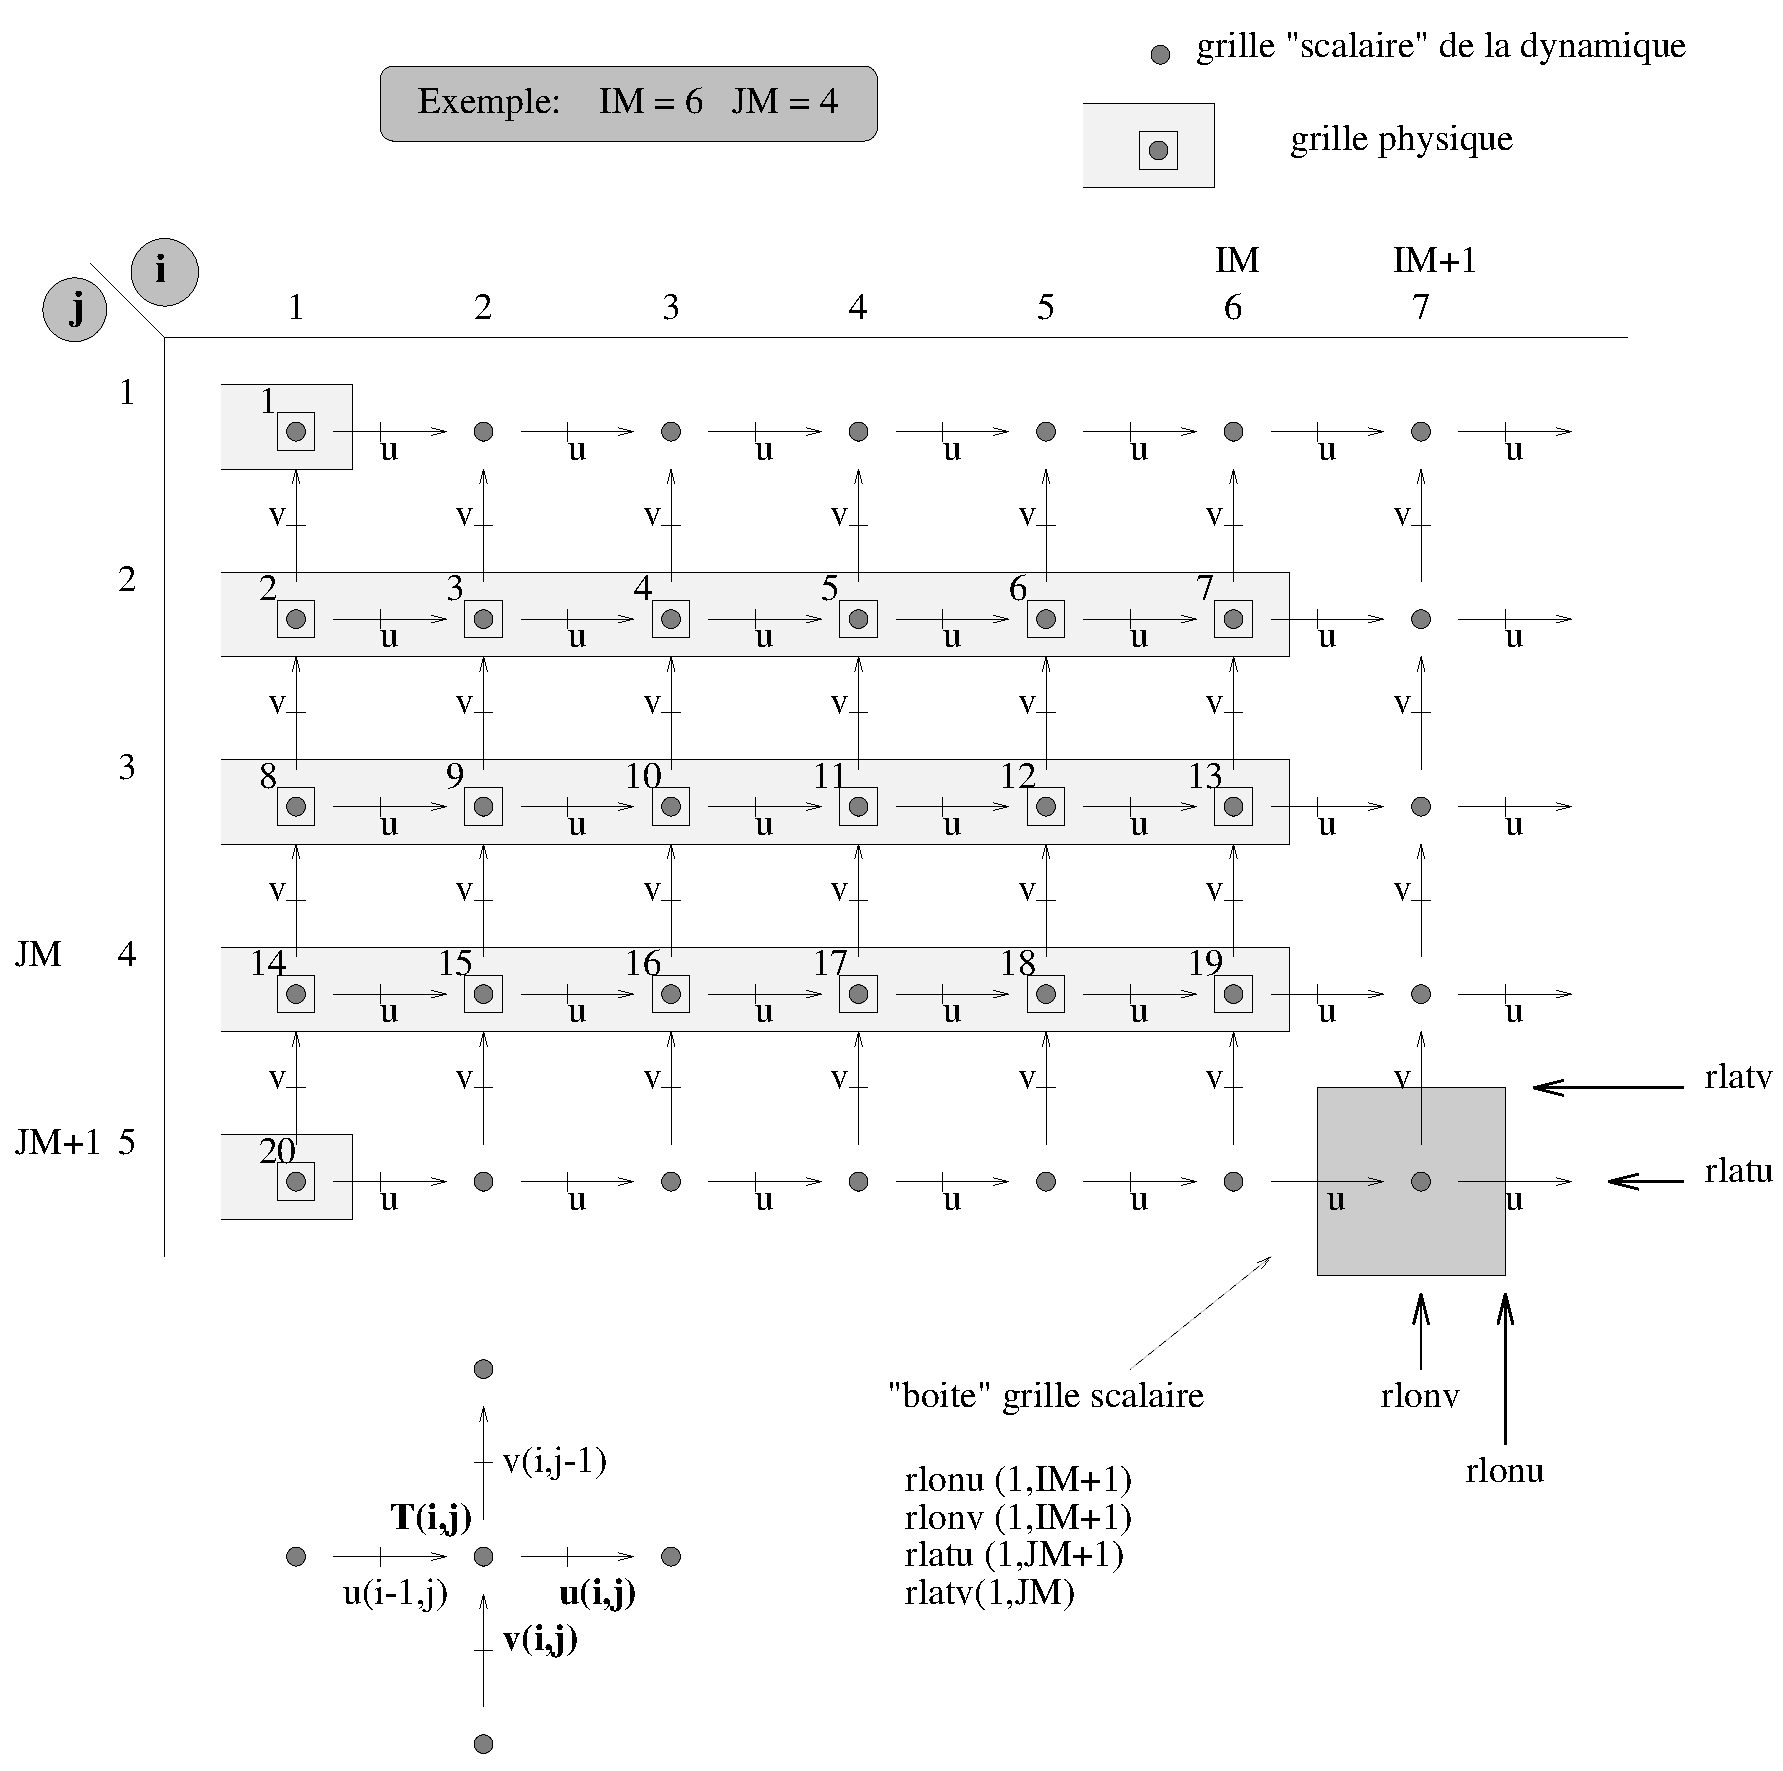
\includegraphics[width=1.2\textwidth]{Fig/grid.eps}}}
\caption{Dynamical and physical grids for a 6 $\times$ 7 horizontal resolution.
In the dynamics (but not in the physics) winds u and v are on specific
staggered grids. Other dynamical variables are on the dynamical ``scalar'' grid.
The physics uses the same ``scalar'' grid for all the variables,
except that nodes are indexed in a single vector containing
NGRID=2+(JM-1)$\times$IM points when counting from the north pole.
N.B.: In the Fortran program, the following variables are used:
 {\tt iim=IM , iip1=IM+1, jjm=JM , jjp1=JM+1}.\label{fg:grid}}
\end{figure}


Dynamics and physics use different grids.
Figure~\ref{fg:grid} shows the correspondence and indexing
of the physical and dynamical grids
as well as the different locations of variables on these grids.
To identify the coordinates of a variable (at one grid point up,
down, right or left)
we use coordinates {\tt rlonu}, {\tt rlatu},
 {\tt rlonv}, {\tt rlatv} (longitudes and
latitudes, in {\bf radians}).

On the dynamical grid, values at {\tt i=1} are the same as at {\tt i=IM+1}
as the latter node is a redundant point (due to the periodicity in longitude,
these two nodes are actualy located at the same place).
Similarly, the extreme {\tt j=1} and {\tt j=JM+1} nodes on the
dynamical grid (respectively corresponding to North and South poles)
are duplicated IM+1 times.\\
In contrast, the physical grid does not contain redundant points
(only one value for each pole and no extra point along longitudes),
as shown in figure~\ref{fg:grid}.
In practice, computations relative to the physics are made
for a series of {\tt ngrid} atmospheric
columns, where {\tt NGRID}={\tt IM}x({\tt JM}-1)+2.

\subsection{Vertical grids}

\begin{figure}[htbp]

{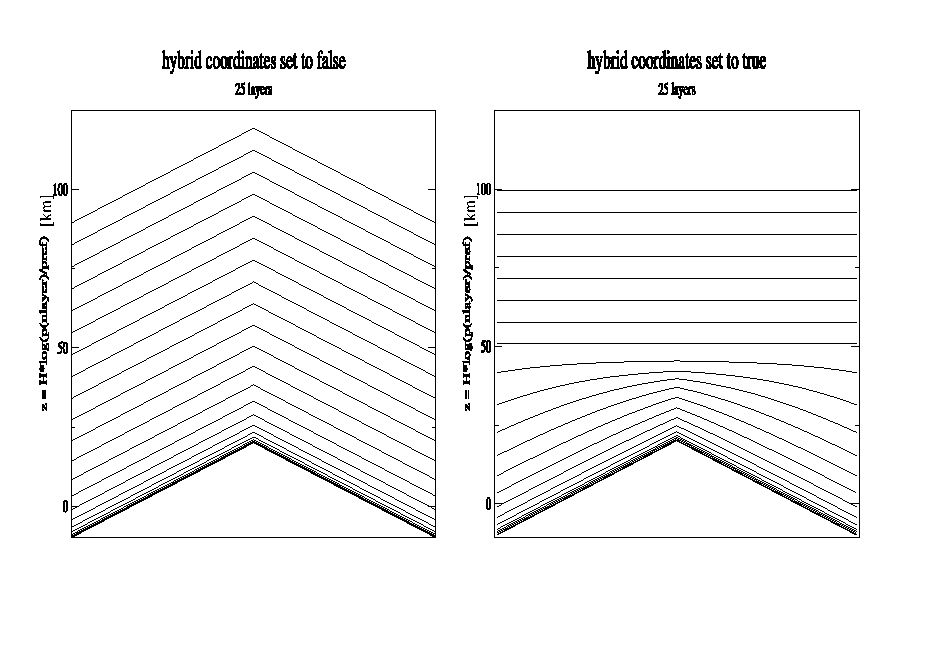
\includegraphics[scale=0.85,clip=true]{Fig/coord.eps}}
\caption[hybrides]
 {Sketch illustrating the difference between hybrid and non-hybrid coordinates}
 \label{fg:hybrid}
\end{figure}


The GCM was initially programmed using sigma coordinates $\sigma = p/ps$
(atmospheric pressure over surface pressure ratio)
which had the advantage of using a constant domain
($\sigma=1$ at the surface and $\sigma=0$ at the top of the atmosphere)
whatever the underlying topography.
However, it is obvious that these coordinates significantly disturb
the stratospheric dynamical representation as the topography is propagated
to the top of the model by the coordinate system.
This problem can elegantly be solved by using a hybrid sigma-P (sigma-pressure)
hybrid coordinate which is equivalent to using $\sigma$ coordinates
near the surface and gradually shifting to purely pressure $p$
coordinates with increasing altitude.
Figure~\ref{fg:hybrid} illustrates the importance of using these
hybrid coordinates compared to simple $\sigma$ coordinates.
The distribution of the vertical layers is irregular,
to enable greater precision at ground level.
In general we use 25 levels to describe the atmosphere to a height of 80 km,
32 levels for simulations up to 120~km, or 50 levels to rise
up to thermosphere.
The first layer describes the first few meters above the ground,
whereas the upper layers span several kilometers.
Figure~\ref{fg:sigma} describes the vertical grid representation
and associated variables.

\begin{figure}
\begin{verbatim}
DYNAMICS                                               PHYSICS
--------                                               -------
[coordinates ap(),bp()]                                [pressures]

ap(llm+1)=0,bp(llm+1)=0  ****************************  plev(nlayer+1)=0
aps(llm),bps(llm)        .. llm .......... nlayer ...  play(nlayer)
ap(llm),bp(llm)          ****************************  plev(nlayer)
aps(llm-1),bps(llm-1)    .. llm-1 ........ nlayer-1 .  play(nlayer-1)
ap(llm-1),bp(llm-1)      ****************************  plev(nlayer-1)
                             :                :
                             :                :
                             :                :
aps(2),bps(2)            ... 2  ............. 2  ....  play(2)
ap(2),bp(2)              ****************************  plev(2)
aps(1),bps(1)            ... 1  ............. 1  ....  play(1)
ap(1)=0,bp(1)=1          **********surface***********  plev(1)=Ps
\end{verbatim}
\caption{Vertical grid description of the {\tt llm (or nlayer)}
atmospheric layers
in the programming code ({\tt llm} is the variable used in the dynamical part,
and {\tt nlayer} is used in the physical part).
Variables {\tt ap, bp} and {\tt aps, bps} indicate the hybrid levels at
the interlayer levels and at middle of the layers respectively.
Pressure at the interlayer is  $Plev(l)=ap(l)+bp(l) \times Ps$ and pressure
in the middle of the layer is defined by $Play(l)=aps(l)+bps(l) \times Ps$,
(where $Ps$ is surface pressure).
Sigma coordinates are merely a specific case of hybrid
coordinates such that $aps=0$ and $bps=P/Ps$.
Note that for the hybrid coordinates, $bps=0$ above $\sim50$~km, leading to
purely pressure levels.
The user can choose whether to run the model using hybrid coordinates or not
by setting variable {\tt hybrid} in run.def to True or False.}
\label{fg:sigma}
\end{figure}

\section{Variables used in the model}

\subsection{Dynamical variables}
The dynamical state variables are the atmospheric temperature,
surface pressure, winds and tracer concentrations.
In practice, the formulation selected to solve the equations in
the dynamics %(see chapter~\ref{sc:dynamic})
is optimised using the following less ``natural'' variables:

\begin{description}
\item - {\bf potential temperature} $\theta$ ({\tt teta} in the code),
linked to temperature {\bf T} by $\theta = T{(P/Pref)}^{-\kappa}$
with $\kappa = R/C_p$
(note that $\kappa$ is called {\tt kappa} in the dynamical code, and {\tt rcp}
in the physical code). We take $Pref=610$ Pa on  Mars.
\item - {\bf surface pressure} ({\tt ps} in the code).
\item - {\bf mass} the atmosphere mass in each grid box ({\tt masse}
in the code).
\item - {\bf the covariant meridional and zonal winds}
{\tt ucov} and {\tt vcov}.
These variables are linked to the "natural" winds by
\verb+ucov = cu * u+ and \verb+vcov = cv * v+, where
\verb+cu+ and \verb+cv+ are constants that only depend on the latitude.
%(see Appendix A).
\item - {\bf mixing ratio of tracers} in the atmosphere, typically
expressed in kg/kg (array {\tt q} in the code).
\end{description}

{\tt ucov} and {\tt vcov}, ``vectorial'' variables, are stored on
``scalari'' grids u and v respectively, in the dynamics
(see section \ref{fg:grid}).
{\tt teta}, {\tt q}, {\tt ps}, {\tt masse}, ``scalar variables'',
are stored on the ``scalar'' grid of the dynamics.



\subsection{Physical variables}

In the physics, the state variables of the dynamics are transmitted
via an interface that interpolates the winds on the scalar grid
(that corresponds to the physical grid) and transforms the dynamical variables
into more ``natural'' variables.
Thus we have winds {\bf u} and  {\bf v} (m.s$^{-1}$),
temperature {\bf T} (K), pressure at the middle of the layers
{\bf play} (Pa) and at interlayers {\bf plev} (Pa), tracers
{\bf q}, etc. (kg/kg) on the same grid.

Furthermore, the physics also handle the evolution of the purely
physical state variables:
\begin{description}
\item - {\bf tsurf} surface temperature (K)
\item - {\bf tsoil} temperature at different layers under the surface (K)
\item - {\bf emis} surface emissivity
\item - {\bf alb} surface albedo
\item - {\bf q2} wind variance, or more precisely the square root of
the turbulent kinetic energy
\item - {\bf qsurf} tracer on the surface (kg.m$^{-2}$)
\item - {\bf rnat} surface type (0 = ocean, 1 = continent)
\item - {\bf beta} surface wetness (0 $\to$ 1 implies dry $\to$ saturated)
\item - [anything else?]
\end{description}

\subsection{Tracers}
The model may include different types of tracers:
\begin{description}
\item - condensed species (e.g., CO$_2$, H$_2$O, dust)
\item - chemically active species (in principle only at the moment)
\item - radiatively active gases (e.g., water vapor)
\end{description}

In the code, all tracers are stored in one three-dimensional array {\tt q},
the third index of which corresponds to each individual tracer.
In input and output files (``start.nc'', ``startfi.nc'',
see Section~\ref{loc:contact1}) tracers are stored separately using their
individual names. Loading specific tracers requires that
the approriate tracer names are set in the {\tt traceur.def} file
(see Section~\ref{sc:traceur.def}), and specific computations
for given tracers (e.g. computing the water or CO$_2$ cycles) 
is controlled by setting the corresponding options in the
{\tt callphys.def} file (see Section~\ref{sc:callphys.def}).

